%% Slides: Towards a Cartography of Datacentering
%% Research Policy 11th Online ECR Conference, 27 April 2026
%% Restructured around DCD corpus EDA + city2graph + visual register

\documentclass[aspectratio=169,11pt]{beamer}
\usetheme{metropolis}

%% IBM Plex fonts
\usepackage[sfdefault,light]{plex-sans}
\usepackage{plex-mono}
\renewcommand{\familydefault}{\sfdefault}
\usepackage{microtype}

\usepackage{booktabs}
\usepackage{tabularx}
\usepackage{array}
\usepackage{tikz}
\usepackage{graphicx}
\usepackage{fontawesome5}
\usepackage{colortbl}
\usepackage{xcolor}
\usetikzlibrary{arrows.meta,positioning,shapes.geometric,fit,backgrounds,calc}

%% B&W Carbon palette
\definecolor{dcblue}{RGB}{22,22,22}
\definecolor{dcaccent}{RGB}{22,22,22}
\definecolor{dclightblue}{RGB}{218,218,218}
\definecolor{dcgray}{RGB}{110,110,110}
\definecolor{dchighlight}{RGB}{192,80,77}   %% red accent for key findings

\setbeamercolor{frametitle}{bg=black!88,fg=white}
\setbeamercolor{progress bar}{fg=black!55}
\setbeamercolor{alerted text}{fg=dchighlight}
\setbeamercolor{example text}{fg=black!70}
\setbeamercolor{normal text}{fg=black!88,bg=white}
\setbeamercolor{background canvas}{bg=white}
\setbeamerfont{alerted text}{series=\bfseries}
\setbeamerfont{frametitle}{size=\normalsize,series=\bfseries}
\setbeamerfont{title}{size=\large,series=\bfseries}
\setbeamerfont{subtitle}{size=\normalsize,series=\mdseries}
\setbeamerfont{institute}{size=\footnotesize,series=\mdseries}
\setbeamerfont{date}{size=\footnotesize,series=\mdseries}
\setbeamerfont{block title}{size=\small,series=\bfseries}

\setbeamersize{text margin left=6mm, text margin right=6mm}
\hfuzz=5pt

\newcommand{\icon}[1]{\textcolor{dcblue}{\faIcon{#1}}\enspace}
\newcommand{\iconfull}[2]{\textcolor{#1}{\faIcon{#2}}}
\newcommand{\highlight}[1]{\textcolor{dchighlight}{\textbf{#1}}}

%% Pipeline step box
\newcommand{\pipestep}[2]{%
  \begin{tikzpicture}
    \node[draw=black!30,rounded corners=2pt,fill=black!4,
          inner sep=4pt,text width=2.6cm,align=center,font=\scriptsize]{%
      \textbf{#1}\\[2pt]#2};
  \end{tikzpicture}%
}

\title{Towards a Cartography of Datacentering}
\subtitle{Trade press, urban graphs, and the visual register of infrastructure}
\author{Babajide Owoyele}
\institute{Erasmus University Rotterdam}
\date{Research Policy ECR Conference \\ 27 April 2026}

\setbeameroption{hide notes}

%% ==================================================================
\begin{document}

%% ------------------------------------------------------------------
%% SLIDE 1 — Title
\begin{frame}[shrink=4]
\titlepage
\end{frame}
\note{15 minutes. I'm going to show you a pipeline, not just a proposal. What does the data center literature actually look like? What does the news record show? What do the urban graphs reveal? And what does the visual register tell us that the text cannot?}

%% ------------------------------------------------------------------
%% SLIDE 2 — The blind spot (brief)
\begin{frame}{\iconfull{dcblue}{search}\enspace One Search. One Blind Spot.}
\begin{columns}[T]
\begin{column}{0.50\textwidth}
  \vspace{0.4em}
  \footnotesize
  \begin{tabular}{@{}lr@{}}
    \toprule
    \textbf{Field} & \textbf{Papers} \\
    \midrule
    Technical efficiency  & ${\gg}90\%$ of corpus \\
    Environmental impact  & ${\approx}11\%$ \\
    STS / geography / media & substantial$^\dagger$ \\
    \midrule
    \alert{Sociotechnical regimes} & \alert{\textbf{0}} \\
    \alert{MLP / TIS / SNM}       & \alert{\textbf{0}} \\
    \bottomrule
  \end{tabular}
  \vspace{0.5em}

  \footnotesize $^\dagger$\,dispersed across media studies, geography,\\
  anthropology venues — not ``data centre'' in title

  \vspace{0.4em}
  \scriptsize\textcolor{dcgray}{Source: OpenAlex API, \texttt{title.search:"data centre"},\\
  2010--2025, $n = 4{,}805$ (UK spelling)}
\end{column}
\begin{column}{0.46\textwidth}
  \vspace{0.6em}
  \small\textbf{The gap is not social science.}\\[0.3em]
  \footnotesize
  Critical data center studies exists\\
  (Edwards et al.\ 2025; Monstadt \& Saltzman 2025).\\[0.4em]
  The gap is \textit{transition governance vocabulary}:\\
  who is responsible, to whom, under what\\
  regulatory structure, and why does the same\\
  level of community contestation produce\\
  a moratorium in Amsterdam but nothing\\
  in Northern Virginia?\\[0.4em]
  \highlight{That is a Research Policy question.}
\end{column}
\end{columns}
\note{Quick, 90 seconds. The bibliometric finding stands but I want to be precise: it's not that social scientists haven't looked at data centers. They have. The gap is the transition governance vocabulary — MLP, TIS, SNM — that would let us explain why governance responses vary. That's what this paper is trying to provide.}
\end{frame}

%% ------------------------------------------------------------------
%% SLIDE 3 — The source: DCD
\begin{frame}{\iconfull{dcblue}{newspaper}\enspace The Primary Record: Data Center Dynamics}
\begin{columns}[T]
\begin{column}{0.52\textwidth}
  \small\textbf{Why trade press as a primary source?}\\[0.4em]
  \footnotesize
  Academic literature misses the granular event record:\\[0.2em]
  \begin{itemize}
    \item Planning disputes filed at county level
    \item Moratoriums negotiated with named operators
    \item Grid connection denials, noise ordinances
    \item Community campaigns before they reach courts
  \end{itemize}
  \vspace{0.4em}
  DCD covers all of this. Systematically. Since 2007.
\end{column}
\begin{column}{0.44\textwidth}
  \vspace{0.3em}
  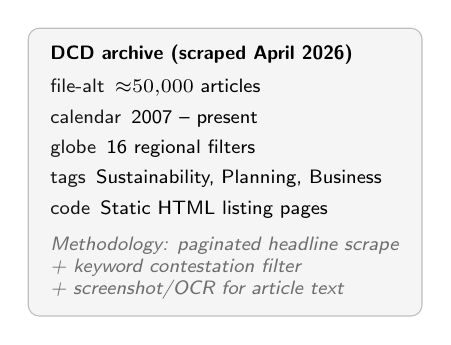
\begin{tikzpicture}[font=\scriptsize]
    \node[draw=black!25,rounded corners,fill=black!4,
          inner xsep=8pt,inner ysep=6pt,align=left] {
      \textbf{DCD archive (scraped April 2026)}\\[4pt]
      \iconfull{dcblue}{file-alt}\enspace ${\approx}50{,}000$ articles\\[3pt]
      \iconfull{dcblue}{calendar}\enspace 2007 -- present\\[3pt]
      \iconfull{dcblue}{globe}\enspace 16 regional filters\\[3pt]
      \iconfull{dcblue}{tags}\enspace Sustainability, Planning, Business\\[3pt]
      \iconfull{dcblue}{code}\enspace Static HTML listing pages\\[5pt]
      \textcolor{dcgray}{\textit{Methodology: paginated headline scrape}}\\
      \textcolor{dcgray}{\textit{+ keyword contestation filter}}\\
      \textcolor{dcgray}{\textit{+ screenshot/OCR for article text}}
    };
  \end{tikzpicture}
\end{column}
\end{columns}
\note{The key methodological point: DCD listing pages are publicly accessible and statically rendered. We scrape headlines, dates, URLs across all 1,723 pages. Individual article pages require Playwright screenshots + OCR. The listing pages alone give us the event record — headline + date + location signals in the headline.}
\end{frame}

%% ------------------------------------------------------------------
%% SLIDE 4 — The pipeline
\begin{frame}[shrink=5]{\iconfull{dcblue}{project-diagram}\enspace The Analytical Pipeline}
\vspace{0.2em}
\begin{center}
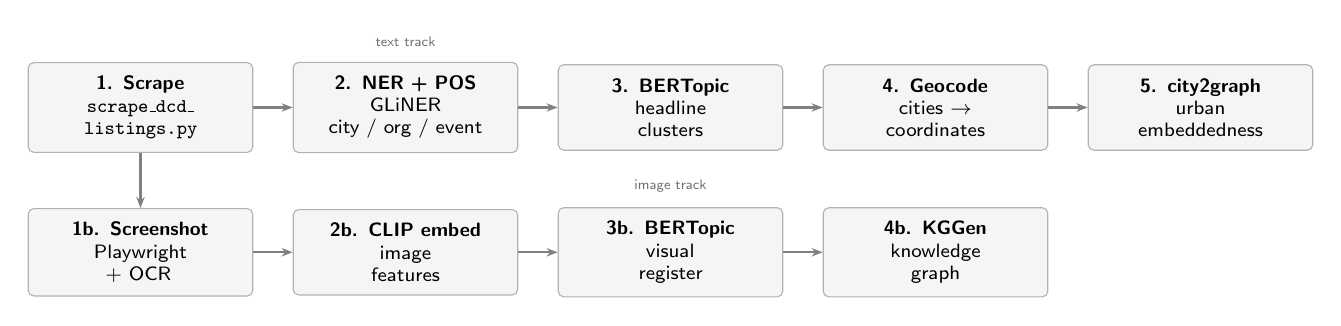
\begin{tikzpicture}[
  node distance=0.35cm and 0.5cm,
  box/.style={draw=black!30,rounded corners=2pt,fill=black!4,
              inner sep=5pt,text width=2.5cm,align=center,font=\scriptsize},
  arr/.style={-{Stealth[length=4pt]},black!50,thick},
  label/.style={font=\tiny,text=dcgray,align=center}
]
  \node[box] (scrape)  {\textbf{1. Scrape}\\\texttt{scrape\_dcd\_}\\\texttt{listings.py}};
  \node[box,right=of scrape] (ner)    {\textbf{2. NER + POS}\\GLiNER\\city / org / event};
  \node[box,right=of ner]    (topic)  {\textbf{3. BERTopic}\\headline\\clusters};
  \node[box,right=of topic]  (geo)    {\textbf{4. Geocode}\\cities $\to$\\coordinates};
  \node[box,right=of geo]    (c2g)    {\textbf{5. city2graph}\\urban\\embeddedness};

  \node[box,below=0.7cm of scrape] (ss)   {\textbf{1b. Screenshot}\\Playwright\\+ OCR};
  \node[box,right=of ss]           (clip) {\textbf{2b. CLIP embed}\\image\\features};
  \node[box,right=of clip]         (vri)  {\textbf{3b. BERTopic}\\visual\\register};
  \node[box,right=of vri]          (kggen) {\textbf{4b. KGGen}\\knowledge\\graph};

  \draw[arr] (scrape) -- (ner);
  \draw[arr] (ner)    -- (topic);
  \draw[arr] (topic)  -- (geo);
  \draw[arr] (geo)    -- (c2g);

  \draw[arr] (scrape) -- (ss);
  \draw[arr] (ss)     -- (clip);
  \draw[arr] (clip)   -- (vri);
  \draw[arr] (vri)    -- (kggen);

  \node[label,above=2pt of ner]   {text track};
  \node[label,above=2pt of vri]   {image track};
\end{tikzpicture}
\end{center}
\vspace{0.1em}
\footnotesize\textcolor{dcgray}{%
  GLiNER: zero-shot NER.\enspace
  BERTopic: topic modelling (text + multimodal CLIP).\enspace
  KGGen: knowledge graph extraction.\enspace
  city2graph: urban graph from Overture Maps.}
\note{Two parallel tracks from the same corpus: text NER + BERTopic identifies who, where, what type of event. Image track: Playwright screenshots, CLIP embeddings, BERTopic multimodal clusters reveal the visual register — what operators and trade press choose to show.}
\end{frame}

%% ------------------------------------------------------------------
%% SLIDE 5 — EDA: Geography
\begin{frame}[shrink=5]{\iconfull{dcblue}{map-marker-alt}\enspace Where Is Contestation?}
\begin{columns}[T]
\begin{column}{0.56\textwidth}
  \includegraphics[width=\textwidth,height=0.72\textheight,keepaspectratio]%
    {../figures/dcd_eda_geography}
\end{column}
\begin{column}{0.40\textwidth}
  \vspace{0.8em}
  \small\textbf{Preliminary findings}\\[0.4em]
  \footnotesize
  \begin{itemize}
    \item US dominates by volume —\\
          planning system is more\\
          granular and public
    \item European events concentrated\\
          in NL, IE, UK, DE
    \item \highlight{Case study cities appear}\\
          \highlight{with high frequency}
    \item Full corpus (1,723 pages)\\
          will reveal temporal clusters
  \end{itemize}
  \vspace{0.4em}
  \textcolor{dcgray}{\scriptsize Preliminary: 5 pages scraped.\\ Full scrape running overnight.\\
  NER (GLiNER) will replace\\headline regex extraction.}
\end{column}
\end{columns}
\note{This is from 5 pages — 112 articles, 22 contestation events. Already showing the US/Europe split. The full corpus with GLiNER NER will give us proper city extraction, not regex.}
\end{frame}

%% ------------------------------------------------------------------
%% SLIDE 6 — EDA: Event types
\begin{frame}{\iconfull{dcblue}{tags}\enspace What Triggers Contestation?}
\begin{columns}[T]
\begin{column}{0.56\textwidth}
  \includegraphics[width=\textwidth,height=0.72\textheight,keepaspectratio]%
    {../figures/dcd_eda_event_types}
\end{column}
\begin{column}{0.40\textwidth}
  \vspace{0.8em}
  \small\textbf{Event type taxonomy}\\[0.4em]
  \footnotesize
  From headline NER + POS:\\[0.3em]
  \begin{tabular}{@{}ll@{}}
    \iconfull{dcblue}{gavel}       & Planning decisions \\[0.2em]
    \iconfull{dcblue}{ban}         & Moratoriums \\[0.2em]
    \iconfull{dcblue}{users}       & Community opposition \\[0.2em]
    \iconfull{dcblue}{bolt}        & Energy / grid \\[0.2em]
    \iconfull{dcblue}{tint}        & Water \\[0.2em]
    \iconfull{dcblue}{balance-scale} & Legal / court \\
  \end{tabular}
  \vspace{0.4em}
  \footnotesize BERTopic will surface\\
  latent topic structure\\
  beyond manual taxonomy.
\end{column}
\end{columns}
\note{The event type taxonomy is preliminary — built from regex on headlines. BERTopic on the full article text (once OCR runs) will give us the latent topic structure. Key question: are energy-grid events and planning events the same cluster or separate? Does community opposition cluster with noise or with water?}
\end{frame}

%% ------------------------------------------------------------------
%% SLIDE 7 — EDA: Timeline
\begin{frame}{\iconfull{dcblue}{chart-line}\enspace Contestation Over Time}
\begin{columns}[T]
\begin{column}{0.62\textwidth}
  \includegraphics[width=\textwidth,height=0.72\textheight,keepaspectratio]%
    {../figures/dcd_eda_timeline}
  \vspace{0.1em}
  \scriptsize\textcolor{dcgray}{Preliminary: 5 pages = most recent 5 days. Full 2007--2026 archive running.}
\end{column}
\begin{column}{0.34\textwidth}
  \vspace{0.8em}
  \small\textbf{What we expect to see}\\[0.4em]
  \footnotesize
  With full corpus (2007--2026):\\[0.3em]
  \begin{itemize}
    \item Pre-2016: near-zero\\
          contestation coverage
    \item 2016--2019: rising\\
          energy + planning events
    \item \highlight{2019: Amsterdam}\\
          \highlight{moratorium onset}
    \item 2020--: community\\
          opposition normalises
    \item 2022--: AI build-out\\
          triggers new wave
  \end{itemize}
\end{column}
\end{columns}
\note{The timeline figure will be the most powerful once the full scrape runs. Expecting a clear phase transition around 2019 and another around 2022-23 with the AI build-out. The Amsterdam moratorium should be visible as an anomaly in an otherwise flat European signal.}
\end{frame}

%% ------------------------------------------------------------------
%% SLIDE 8 — city2graph: from corpus to urban graph
\begin{frame}[shrink=8]{\iconfull{dcblue}{city}\enspace From Corpus to Urban Graph}
\begin{columns}[T]
\begin{column}{0.50\textwidth}
  \includegraphics[width=\textwidth,height=0.68\textheight,keepaspectratio]%
    {../figures/wp3_urban_graphs_map}
\end{column}
\begin{column}{0.46\textwidth}
  \vspace{0.4em}
  \small\textbf{Pipeline: corpus cities $\to$ graphs}\\[0.4em]
  \footnotesize
  \begin{enumerate}
    \item GLiNER extracts city names\\
          from DCD headlines + OCR text
    \item Top N cities geocoded
    \item city2graph pulls Overture Maps\\
          for each city bounding box
    \item Graph: data center node\\
          $\leftrightarrow$ power, residential,\\
          commercial neighbours
    \item Compare: residential adjacency,\\
          power node density, graph topology
  \end{enumerate}
  \vspace{0.4em}
  \footnotesize\textbf{Seed result (3 cities):}\\[0.2em]
  \begin{tabular}{@{}lrr@{}}
    & Res.\ zones & Power nodes \\
    \midrule
    Ashburn  & 1  & 36 \\
    Amsterdam & 61 & 2  \\
    Dublin   & 361 & 6  \\
  \end{tabular}
\end{column}
\end{columns}
\note{The pipeline scales: GLiNER gives us the city list from the corpus, city2graph builds the urban graphs. The structural difference — Ashburn isolated, Amsterdam embedded — is not just a planning story. It's a spatial story. The graph makes it systematic rather than impressionistic.}
\end{frame}

%% ------------------------------------------------------------------
%% SLIDE 9 — Visual register
\begin{frame}[shrink=5]{\iconfull{dcblue}{images}\enspace The Visual Register of Datacentering}
\begin{columns}[T]
\begin{column}{0.50\textwidth}
  \small\textbf{What does DCD show?}\\[0.4em]
  \footnotesize
  Following Jancsary et al.\ (2015):\\
  institutions are accomplished\\
  through visual grammar.\\[0.4em]
  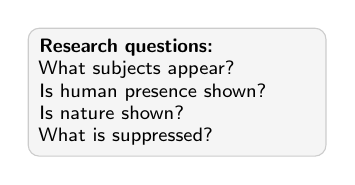
\begin{tikzpicture}[font=\scriptsize,node distance=0.25cm]
    \node[draw=black!20,rounded corners,fill=black!4,
          inner sep=4pt,text width=3.5cm] (q) {
      \textbf{Research questions:}\\
      What subjects appear?\\
      Is human presence shown?\\
      Is nature shown?\\
      What is suppressed?
    };
  \end{tikzpicture}
  \vspace{0.3em}

  \textbf{Pipeline:}\\[0.2em]
  \footnotesize
  Playwright screenshot $\to$ image extract\\
  $\to$ CLIP embed $\to$ BERTopic clusters\\
  $\to$ Visual Register Index (VRI)\\[0.3em]
  Run on 24GB GPU via Gemma~4 + Ollama\\
  for richer caption-level description.
\end{column}
\begin{column}{0.46\textwidth}
  \vspace{0.3em}
  \small\textbf{Expected clusters}\\[0.3em]
  \footnotesize
  \begin{tabular}{@{}ll@{}}
    \toprule
    \textbf{Visual type} & \textbf{Register function} \\
    \midrule
    Server hall interior & Technical sublime \\
    Exterior + landscape & Naturalisation \\
    Workers / people     & Labour legitimacy \\
    Renewable energy     & Green imaginary \\
    Blank / exterior only & Strategic invisibility \\
    \bottomrule
  \end{tabular}
  \vspace{0.4em}
  \footnotesize Compare: DCD editorial\\
  images vs operator corporate\\
  imagery (WP2 ECI pipeline)\\[0.3em]
  \highlight{What is shown in news $\neq$}\\
  \highlight{what is shown on websites}
\end{column}
\end{columns}
\note{The visual register is the newest strand. BERTopic has a multimodal mode using CLIP embeddings — same topic modelling approach but on images. We'll run this on DCD article screenshots and compare to corporate imagery. The hypothesis: DCD shows more contested and material imagery; corporate sites show landscapes and renewables.}
\end{frame}

%% ------------------------------------------------------------------
%% SLIDE 10 — Datacentering: what ties it together
\begin{frame}{\iconfull{dcblue}{link}\enspace Datacentering: The Concept}
\begin{columns}[T]
\begin{column}{0.52\textwidth}
  \vspace{0.3em}
  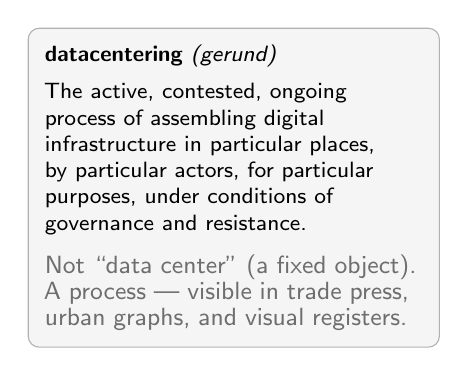
\begin{tikzpicture}[font=\footnotesize,node distance=0.3cm and 0.1cm]
    \node[draw=black!30,rounded corners,fill=black!4,
          inner sep=6pt,text width=4.8cm,align=left] {
      \textbf{datacentering} \textit{(gerund)}\\[4pt]
      The active, contested, ongoing\\
      process of assembling digital\\
      infrastructure in particular places,\\
      by particular actors, for particular\\
      purposes, under conditions of\\
      governance and resistance.\\[6pt]
      \textcolor{dcgray}{\small Not ``data center'' (a fixed object).}\\
      \textcolor{dcgray}{\small A process — visible in trade press,}\\
      \textcolor{dcgray}{\small urban graphs, and visual registers.}
    };
  \end{tikzpicture}
\end{column}
\begin{column}{0.44\textwidth}
  \small\textbf{Three analytical registers}\\[0.4em]
  \footnotesize
  \begin{tabular}{@{}ll@{}}
    \toprule
    \textbf{What} & \textbf{Where it lives} \\
    \midrule
    Textual imaginary & ECI, NER, BERTopic \\
    Spatial structure & city2graph, ownership \\
    Visual grammar & CLIP, BERTopic-MM \\
    \bottomrule
  \end{tabular}
  \vspace{0.4em}
  \footnotesize Each register reveals a\\
  different dimension of how\\
  infrastructure is made\\
  \textit{legible} or \textit{invisible}.\\[0.4em]
  The corpus makes this\\
  systematic and scalable.
\end{column}
\end{columns}
\note{The concept pulls the three empirical strands together. Datacentering as a gerund — a process — is why we need a corpus approach. Each article in DCD is an instance of datacentering being contested, negotiated, or naturalised. The pipeline reads the corpus; the concept interprets it.}
\end{frame}

%% ------------------------------------------------------------------
%% SLIDE 11 — The Cartalog
\begin{frame}[shrink=3]{\iconfull{dcblue}{map}\enspace The Cartalog: A Cartographic Catalog}
\begin{columns}[T]
\begin{column}{0.52\textwidth}
  \small\textbf{What we are building}\\[0.4em]
  \footnotesize
  Not just a spreadsheet — a \textit{navigable map}:\\[0.3em]
  \begin{itemize}
    \item Each facility as a spatial entry
    \item Linked to: contestation events\\
          (DCD corpus), ownership network,\\
          urban graph, ECI, visual register
    \item Community-editable (CC BY 4.0)
    \item Versioned (git-backed)
    \item Open pipelines: GLiNER, BERTopic,\\
          city2graph, KGGen
  \end{itemize}
  \vspace{0.3em}
  \texttt{\small github.com/babayyy/cartalog}
\end{column}
\begin{column}{0.44\textwidth}
  \vspace{0.3em}
  \small\textbf{Concrete asks}\\[0.4em]
  \footnotesize
  \begin{itemize}
    \item \icon{database}Local planning records,\\
          dispute documents
    \item \icon{globe}Non-English corpus:\\
          NL, DE, FR, IE planning records
    \item \icon{network-wired}Company registry\\
          or REIT data access
    \item \icon{code}Replication in\\
          other jurisdictions
    \item \icon{comments}Methodological\\
          critique — especially on\\
          contestation classification
  \end{itemize}
\end{column}
\end{columns}
\note{The cartalog is the open infrastructure. It is also theoretically motivated — if datacentering is CAS-like, the cartography must be distributed. The pipeline is the contribution: anyone can run it on their jurisdiction. Come build it.}
\end{frame}

%% ==================================================================
%% APPENDIX — Q&A backup slides
%% ==================================================================
\appendix

\begin{frame}[noframenumbering]{\faIcon{question-circle}\enspace Q: Why trade press and not planning documents directly?}
\begin{columns}[T]
\begin{column}{0.52\textwidth}
  \small\textbf{DCD as a methodological choice}\\[0.4em]
  \footnotesize
  \begin{itemize}
    \item Planning documents are fragmented across thousands of local authority portals — no unified index
    \item DCD \textit{aggregates} the event record — reporters follow planning submissions across jurisdictions
    \item Listing pages are accessible; planning portals often require login or are behind paywalls
    \item DCD captures \textit{community response} and \textit{media framing} alongside the formal planning event
  \end{itemize}
\end{column}
\begin{column}{0.44\textwidth}
  \small\textbf{Limitations we acknowledge}\\[0.4em]
  \footnotesize
  \begin{itemize}
    \item English-language bias (DCD is primarily Anglophone)
    \item Editorial selection — DCD covers larger operators more than small colo
    \item Not a comprehensive legal record\\
          (some disputes never reach trade press)
  \end{itemize}
  \vspace{0.3em}
  \textcolor{dcgray}{\textit{Mitigation: supplement with GLiNER\\NER on local news + planning records\\where available.}}
\end{column}
\end{columns}
\end{frame}

\begin{frame}[noframenumbering]{\faIcon{question-circle}\enspace Q: Why CAS and not MLP / TIS / SNM?}
\begin{columns}[T]
\begin{column}{0.48\textwidth}
  \small\textbf{Complementary, not competing}\\[0.4em]
  \footnotesize
  MLP excels when a niche is visible and a regime is identifiable. Here:
  \begin{itemize}
    \item No stable niche — hyperscalers \textit{are} the incumbent
    \item Regime boundaries dissolve across planning, energy, finance
    \item Outcomes are emergent — no single actor planned Ashburn
  \end{itemize}
\end{column}
\begin{column}{0.48\textwidth}
  \small\textbf{CAS as sensemaking lens}\\[0.4em]
  \footnotesize
  \begin{itemize}
    \item Emergent outcomes no single actor controls
    \item Non-linear feedback (moratorium $\to$ relocation $\to$ new contestation)
    \item Heterogeneous agents: grids, aquifers, pension funds, planning law
    \item CAS doesn't replace MLP — it flags \textit{why} MLP categories keep slipping
  \end{itemize}
  \textcolor{dcgray}{\textit{Future work: operationalise\\regime boundaries via corpus.}}
\end{column}
\end{columns}
\end{frame}

\begin{frame}[noframenumbering]{\faIcon{question-circle}\enspace Q: Isn't 5 pages too small a sample?}
\small\textbf{Yes — by design for this presentation}\\[0.4em]
\footnotesize
The full 1,723-page scrape is running. What 5 pages already shows:\\[0.4em]
\begin{tabular}{@{}lll@{}}
\toprule
\textbf{Finding} & \textbf{5-page sample} & \textbf{Full corpus} \\
\midrule
Pipeline works & \checkmark\ verified & Scales automatically \\
Geography signal & US + Europe split visible & Full 2007--2026 map \\
Event taxonomy & 6 types identified & BERTopic topic clusters \\
City2graph & 3 seed cities & All cities in corpus \\
Visual register & Method designed & Gemma~4 on GPU \\
\bottomrule
\end{tabular}\\[0.4em]
\textcolor{dcgray}{\textit{The contribution is the pipeline. Sample size scales with compute.}}
\end{frame}

\begin{frame}[noframenumbering]{\faIcon{question-circle}\enspace Q: What is GLiNER? What is KGGen?}
\begin{columns}[T]
\begin{column}{0.48\textwidth}
  \small\textbf{GLiNER}\\[0.3em]
  \footnotesize
  Generalised Linear NER — zero-shot named entity recognition.\\[0.3em]
  Unlike spaCy or BERT fine-tuned models:\\
  \begin{itemize}
    \item No labelled training data needed
    \item Entity types defined at inference time
    \item Works on: city, operator, grid\_operator,\\
          planning\_body, opposition\_group
    \item Runs locally
  \end{itemize}
\end{column}
\begin{column}{0.48\textwidth}
  \small\textbf{KGGen}\\[0.3em]
  \footnotesize
  Knowledge graph generation from unstructured text.\\[0.3em]
  From DCD article text:\\
  \begin{itemize}
    \item Extracts: (operator) $\to$ [applied\_for] $\to$ (planning\_permission)
    \item (community) $\to$ [opposed] $\to$ (facility)
    \item (council) $\to$ [imposed] $\to$ (moratorium)
  \end{itemize}
  Combined with city2graph = spatial + relational graph of the assemblage.
\end{column}
\end{columns}
\end{frame}

\begin{frame}[noframenumbering]{\faIcon{question-circle}\enspace Q: BERTopic for images — how does that work?}
\small\textbf{BERTopic multimodal mode uses CLIP embeddings}\\[0.4em]
\footnotesize
Standard BERTopic: embed text $\to$ cluster $\to$ label clusters.\\
Multimodal BERTopic: same, but with CLIP image embeddings as input.\\[0.5em]
\begin{tabular}{@{}lll@{}}
\toprule
\textbf{Step} & \textbf{Text track} & \textbf{Image track} \\
\midrule
Input  & DCD article headlines / OCR & Extracted article images \\
Embed  & sentence-transformers & CLIP (ViT-B/32) \\
Reduce & UMAP & UMAP \\
Cluster & HDBSCAN & HDBSCAN \\
Label  & KeyBERT terms & Gemma~4 captions (Ollama) \\
Output & Topic: ``moratorium energy grid'' & Topic: ``server hall cooling'' \\
\bottomrule
\end{tabular}\\[0.4em]
\textcolor{dcgray}{\textit{Gemma~4 on 24GB GPU: generates natural-language descriptions of each image cluster, enabling the Visual Register Index.}}
\end{frame}

\end{document}
